\documentclass[a4paper, 14pt]{extarticle}

% Поля
%--------------------------------------
\usepackage{geometry}
\geometry{a4paper,tmargin=2cm,bmargin=2cm,lmargin=3cm,rmargin=1cm}
%--------------------------------------


%Russian-specific packages
%--------------------------------------
\usepackage[T2A]{fontenc}
\usepackage[utf8]{inputenc} 
\usepackage[english, main=russian]{babel}
%--------------------------------------

\usepackage{textcomp}

% Красная строка
%--------------------------------------
\usepackage{indentfirst}               
%--------------------------------------             


%Graphics
%--------------------------------------
\usepackage{graphicx}
\graphicspath{ {./images/} }
\usepackage{wrapfig}
%--------------------------------------

% Полуторный интервал
%--------------------------------------
\linespread{1.3}                    
%--------------------------------------

%Выравнивание и переносы
%--------------------------------------
% Избавляемся от переполнений
\sloppy
% Запрещаем разрыв страницы после первой строки абзаца
\clubpenalty=10000
% Запрещаем разрыв страницы после последней строки абзаца
\widowpenalty=10000
%--------------------------------------

%Списки
\usepackage{enumitem}

%Подписи
\usepackage{caption} 

%Гиперссылки
\usepackage{hyperref}

\hypersetup {
	unicode=true
}

%Рисунки
%--------------------------------------
\DeclareCaptionLabelSeparator*{emdash}{~--- }
\captionsetup[figure]{labelsep=emdash,font=onehalfspacing,position=bottom}
%--------------------------------------

\usepackage{tempora}

%Листинги
%--------------------------------------
\usepackage{listings}
\lstset{
  basicstyle=\ttfamily\footnotesize, 
  %basicstyle=\footnotesize\AnkaCoder,        % the size of the fonts that are used for the code
  breakatwhitespace=false,         % sets if automatic breaks shoulbd only happen at whitespace
  breaklines=true,                 % sets automatic line breaking
  captionpos=t,                    % sets the caption-position to bottom
  inputencoding=utf8,
  frame=single,                    % adds a frame around the code
  keepspaces=true,                 % keeps spaces in text, useful for keeping indentation of code (possibly needs columns=flexible)
  keywordstyle=\bf,       % keyword style
  numbers=left,                    % where to put the line-numbers; possible values are (none, left, right)
  numbersep=5pt,                   % how far the line-numbers are from the code
  xleftmargin=25pt,
  xrightmargin=25pt,
  showspaces=false,                % show spaces everywhere adding particular underscores; it overrides 'showstringspaces'
  showstringspaces=false,          % underline spaces within strings only
  showtabs=false,                  % show tabs within strings adding particular underscores
  stepnumber=1,                    % the step between two line-numbers. If it's 1, each line will be numbered
  tabsize=2,                       % sets default tabsize to 8 spaces
  title=\lstname                   % show the filename of files included with \lstinputlisting; also try caption instead of title
}
%--------------------------------------

%%% Математические пакеты %%%
%--------------------------------------
\usepackage{amsthm,amsfonts,amsmath,amssymb,amscd}  % Математические дополнения от AMS
\usepackage{mathtools}                              % Добавляет окружение multlined
\usepackage[perpage]{footmisc}
%--------------------------------------

%--------------------------------------
%			НАЧАЛО ДОКУМЕНТА
%--------------------------------------

\begin{document}

%--------------------------------------
%			ТИТУЛЬНЫЙ ЛИСТ
%--------------------------------------
\begin{titlepage}
\thispagestyle{empty}
\newpage


%Шапка титульного листа
%--------------------------------------
\vspace*{-60pt}
\hspace{-65pt}
\begin{minipage}{0.3\textwidth}
\hspace*{-20pt}\centering

\includegraphics[width=\textwidth]{emblem}
\end{minipage}
\begin{minipage}{0.67\textwidth}\small \textbf{
\vspace*{-0.7ex}
\hspace*{-6pt}\centerline{Министерство науки и высшего образования Российской Федерации}
\vspace*{-0.7ex}
\centerline{Федеральное государственное бюджетное образовательное учреждение }
\vspace*{-0.7ex}
\centerline{высшего образования}
\vspace*{-0.7ex}
\centerline{<<Московский государственный технический университет}
\vspace*{-0.7ex}
\centerline{имени Н.Э. Баумана}
\vspace*{-0.7ex}
\centerline{(национальный исследовательский университет)>>}
\vspace*{-0.7ex}
\centerline{(МГТУ им. Н.Э. Баумана)}}
\end{minipage}
%--------------------------------------

%Полосы
%--------------------------------------
\vspace{-25pt}
\hspace{-35pt}\rule{\textwidth}{2.3pt}

\vspace*{-20.3pt}
\hspace{-35pt}\rule{\textwidth}{0.4pt}
%--------------------------------------

\vspace{1.5ex}
\hspace{-35pt} \noindent \small ФАКУЛЬТЕТ\hspace{80pt} <<Информатика и системы управления>>

\vspace*{-16pt}
\hspace{47pt}\rule{0.83\textwidth}{0.4pt}

\vspace{0.5ex}
\hspace{-35pt} \noindent \small КАФЕДРА\hspace{50pt} <<Теоретическая информатика и компьютерные технологии>>

\vspace*{-16pt}
\hspace{30pt}\rule{0.866\textwidth}{0.4pt}
  
\vspace{11em}

\begin{center}
\Large {\bf Лабораторная работа № 4} \\
\large {\bf по курсу <<Разработка мобильных приложений>>} \\
\large {\bf <<Приложение выполняющее функцию FTP-клиента,  SSH-клиента и SMTP-клиента>>} \\
\end{center}\normalsize

\vspace{8em}


\begin{flushright}
  {Студентка группы ИУ9-72Б Самохвалова П. С. \hspace*{15pt}\\
  \vspace{2ex}
  Преподаватель Посевин Д. П.\hspace*{15pt}}
\end{flushright}

\bigskip

\vfill
 

\begin{center}
\textsl{Москва 2023}
\end{center}
\end{titlepage}
%--------------------------------------
%		КОНЕЦ ТИТУЛЬНОГО ЛИСТА
%--------------------------------------

\renewcommand{\ttdefault}{pcr}

\setlength{\tabcolsep}{3pt}
\newpage
\setcounter{page}{2}

\section{Задание}\label{Sect::task}

Реализовать мобильное приложение выполняющее функцию FTP-клиента,  SSH-клиента и SMTP-клиента.  В приложении должен быть следующий функционал:

1. Экран с параметрами FTP-подключения, реализованный в виде формы: значения полей FTP-доступа должны храниться постоянно, другими словами после ввода данных при последующем запуске приложения ранее введенные значения полей должны сохраняться и загружаться в поля ввода, если пользователь хочет изменить параметры FTP-доступа, то он редактирует значения соответствующих полей и пересохраняет форму. На отдельном экране необходимо реализовать интерфейс выполнения FTP-команд: вывода содержимого директории, перехода в другую директорию, создания директории, загрузки файла, скачивание файла, результат ответа от FTP-сервера должен записываться в виджет вывода данных под формой ввода команд.

2. Экран с параметрами SSH-подключения, реализованный в виде формы: значения полей SSH-доступа должны храниться постоянно, другими словами после ввода данных при последующем запуске приложения ранее введенные значения полей должны сохраняться и загружаться в поля ввода, если пользователь хочет изменить параметры SSH-доступа, то он редактирует значения соответствующих полей и пересохраняет форму. На отдельном экране необходимо реализовать интерфейс выполнения консольных команд выполняемых на SSH-сервере. Результат ответа от SSH-сервера должен записываться в виджет вывода данных под формой ввода команд.

3. Экран с параметрами SMTP-подключения, реализованный в виде формы, значения полей SMTP-аутентификации должны храниться постоянно, другими словами после ввода данных при последующем запуске приложения ранее введенные значения полей должны сохраняться и загружаться в поля ввода, если пользователь хочет изменить параметры smtp-аутентификации, то он редактирует значения соответствующих полей и пересохраняет форму. На отдельном экране необходимо реализовать форму отправки письма, при этом поля формы должны состоять из полей: адрес электронной почты, тема письма, сообщение. Результат ответа от SMTP-сервера должен записываться в виджет вывода данных под формой ввода команд.

\section{Практическая реализация}\label{Sect::code}

Исходный код программы представлен в листинге~\ref{lst:code1}.

\begin{lstlisting}[language={},caption={FTP-клиент,  SSH-клиент и SMTP-клиент},label={lst:code1}]
import 'package:flutter/material.dart';
import 'ftp_filelist_screen.dart';
import 'package:shared_preferences/shared_preferences.dart';
import 'dart:io';

class MyApp extends StatelessWidget {
  @override
  Widget build(BuildContext context) {
    return MaterialApp(
      home: FTPScreen(),
    );
  }
}

class FTPScreen extends StatefulWidget {
  @override
  _FTPScreenState createState() => _FTPScreenState();
}

class _FTPScreenState extends State<FTPScreen> {
  late TextEditingController _ftpHostController = TextEditingController();
  late TextEditingController _ftpUsernameController = TextEditingController();
  late TextEditingController _ftpPasswordController = TextEditingController();
  // late TextEditingController _ftpPortController = TextEditingController();

  late SharedPreferences _prefs;

  @override
  void initState() {
    super.initState();
    _init();
  }

  void _init() async {
    _prefs = await SharedPreferences.getInstance();
    _initTextControllers();
  }

  void _initTextControllers() {
    _ftpHostController.text = _prefs.getString('ftpHost') ?? '';
    _ftpUsernameController.text = _prefs.getString('ftpUsername') ?? '';
    _ftpPasswordController.text = _prefs.getString('ftpPassword') ?? '';
    // _ftpPortController.text = _prefs.getString('ftpPort') ?? '';
  }

  void _saveFtpSettings() {
    _prefs.setString('ftpHost', _ftpHostController.text);
    _prefs.setString('ftpUsername', _ftpUsernameController.text);
    _prefs.setString('ftpPassword', _ftpPasswordController.text);
    // _prefs.setString('ftpPort', _ftpPortController.text);
    ScaffoldMessenger.of(context).showSnackBar(
      SnackBar(content: Text('FTP settings saved')),
    );
  }

  void _navigateToFTPCommandsScreen() {
    String host = _ftpHostController.text;
    String username = _ftpUsernameController.text;
    String password = _ftpPasswordController.text;
    // String port = _ftpPortController.text;

    Navigator.push(
      context,
      MaterialPageRoute(
        builder: (context) => FileListScreen(
          server: host,
          login: username,
          password: password,
          // port: port,
        ),
      ),
    );
  }

  @override
  Widget build(BuildContext context) {
    return Scaffold(
      appBar: AppBar(
        title: Text('FTP Data Entry Form'),
      ),
      body: Padding(
        padding: EdgeInsets.all(16.0),
        child: Column(
          mainAxisAlignment: MainAxisAlignment.center,
          children: <Widget>[
            TextField(
              controller: _ftpHostController,
              decoration: InputDecoration(labelText: 'FTP Server'),
            ),
            TextField(
              controller: _ftpUsernameController,
              decoration: InputDecoration(labelText: 'FTP Login'),
            ),
            TextField(
              controller: _ftpPasswordController,
              decoration: InputDecoration(labelText: 'FTP Password'),
            ),
            // TextField(
            //   controller: _ftpPortController,
            //   decoration: InputDecoration(labelText: 'FTP Port'),
            // ),
            SizedBox(height: 10),
            ElevatedButton(
              onPressed: _saveFtpSettings,
              child: Text('Save'),
            ),
            SizedBox(height: 10),
            ElevatedButton(
              onPressed: _navigateToFTPCommandsScreen,
              child: Text('Connect to FTP server'),
            ),
          ],
        ),
      ),
    );
  }
}

import 'dart:io';

import 'package:flutter/material.dart';
import 'package:ftpconnect/ftpconnect.dart';
import 'package:file_picker/file_picker.dart';

class FileListScreen extends StatefulWidget {
  final String server;
  final String login;
  final String password;

  FileListScreen(
      {required this.server, required this.login, required this.password});

  @override
  _FileListScreenState createState() =>
      _FileListScreenState(server, login, password);
}

class FTPManager {
  late String _server;
  late String _login;
  late String _password;
  late FTPConnect _ftpConnect;

  List _fileList = [];
  String _currentDir = "";
  // List<String> _currentPath = [];

  List get fileList => _fileList;
  // late List<String> consoleLogs = [];

  int maxLogCount = 4;
  late List<String> consoleLogs = List<String>.generate(
      maxLogCount, (index) => "");

  FTPManager(String server, String login, String password) {
    _server = server;
    _login = login;
    _password = password;
    _ftpConnect =
        FTPConnect(_server, user: _login, pass: _password, showLog: true);
  }

  Function()? _onUpdate;

  void _log(String message) {
    final DateTime now = DateTime.now();
    final String formattedTime = "[${now}] ";
    final formattedMessage = formattedTime + "> " + message;
    consoleLogs.insert(0, formattedMessage);
    if (consoleLogs.length > maxLogCount) {
      consoleLogs.removeLast();
    }
    _onUpdate!();
  }

  void setOnUpdateCallback(Function() onUpdate) {
    _onUpdate = onUpdate;
  }

  Future<void> connect() async {
    try {
      await _ftpConnect.connect();
      _log("Connected to " + _server);
    } catch (error) {
      _log("FTP connection error: " + error.toString());
    }
  }

  Future<void> disconnect() async {
    await _ftpConnect.disconnect();
    _fileList.clear();
    _currentDir = '';
    _log("Disconnected from " + _server);
  }

  Future<void> refreshFTPData(String currentDir) async {
    // _currentPath.add(currentDir);
    print("Refreshing");
    // print(_currentPath.join("/"));
    await _ftpConnect.changeDirectory(currentDir);
    List dirList = await _ftpConnect.listDirectoryContent();
    _fileList = dirList;
    _currentDir = currentDir;
    // for (var file in dirList) {
    //   print('File name: ${file.name}' + 'File type ${file.type}');
    // }
    if (currentDir == "") {
      _log("Refreshing in current directory");
    } else {
      _log("Refreshing in directory: " + currentDir);

    }
  }

  void _openFileExplorer() async {
    FilePickerResult? result = await FilePicker.platform.pickFiles();

    if (result != null) {
      File file = File(result.files.single.path!);
      await uploadFileToFTP(file);
    } else {

    }
  }

  Future<void> uploadFileToFTP(File fileName) async {
    try {
      await _ftpConnect.uploadFile(fileName);
      _log("File ${fileName} has been successfully uploaded to FTP");
      refreshFTPData('');
    } catch (error) {
      _log("FTP upload error: ${error.toString()}");
    }
  }

  Future<void> deleteFileFromFTP(String fileName) async {
    // implementation for deleting file from FTP
    try {
      await _ftpConnect.deleteFile(fileName);
      _log("File: " + fileName + "deleted successfully");
      refreshFTPData('');
    } catch (error) {
      _log("FTP deleting error: " + error.toString());
    }
  }

  Future<void> downloadFileFromFTP(String fileName) async {

    try {
      File localFilePath = File("/home/user1/" + fileName);
      _log("Local path: " + localFilePath.toString());
      await _ftpConnect.downloadFile(fileName, localFilePath);
      _log("File: " + fileName + " downloaded successfully");
    } catch (error) {
      _log("FTP download error: " + error.toString());
    }
  }

  Future<void> createFTPDirectory(String currentDir) async {
    // implementation for creating directory on FTP

    try {
      await _ftpConnect.makeDirectory(currentDir);
      _log("New directory created successfully: " + currentDir);
      refreshFTPData('');
    } catch (error) {
      _log("FTP creating directory error: " + error.toString());
    }
  }
}

class _FileListScreenState extends State<FileListScreen> {
  late String _server;
  late String _login;
  late String _password;
  late FTPManager _ftpManager;

  _FileListScreenState(String server, String login, String password) {
    _server = server;
    _login = login;
    _password = password;
    _ftpManager = FTPManager(_server, _login, _password);
    _ftpManager.setOnUpdateCallback(_onUpdate);
  }

  _onUpdate() {
    setState(() {});
  }

  @override
  void initState() {
    super.initState();
    _ftpManager.connect().then((_) {
      _ftpManager.refreshFTPData('').then((_) {
        _onUpdate();
      });
    });
  }

  @override
  Widget build(BuildContext context) {
    return Scaffold(
      appBar: AppBar(
        title: Text('File List Screen'),
      ),
      body: Column(
        children: [
          // Align(
          //   alignment: Alignment.centerLeft,
          //   child: Text('Current Path: ' + _ftpManager._currentDir),
          // ),

          Expanded(
            child: ListView.builder(
              itemCount: _ftpManager.fileList.length,

              itemBuilder: (context, index) {
                final file = _ftpManager.fileList[index];
                final isDirectory = file.type.toString() == "FTPEntryType.DIR";
                final icon =
                    isDirectory ? Icons.folder : Icons.insert_drive_file;
                final color = isDirectory ? Colors.orange : Colors.grey;

                return ListTile(
                  leading: Icon(icon, color: color),
                  title: Text(file.name),
                  onTap: () async {
                    final currentFile = _ftpManager.fileList[index].name;
                    // final currentPath = _ftpManager._currentPath.join("/");
                    // final path = currentPath.isNotEmpty ? "$currentPath/$currentFile" : currentFile;
                    await _ftpManager.refreshFTPData(currentFile);
                    setState(
                        () {});
                  },
                  onLongPress: () {

                    showMenu(
                      context: context,
                      position: RelativeRect.fromLTRB(0, 0, 0, 0),
                      items: [
                        const PopupMenuItem(
                          value: "download",
                          child: Text("Download file"),
                        ),
                        const PopupMenuItem(
                          value: "delete",
                          child: Text("Delete file"),
                        ),
                      ],
                    ).then((value) {
                      if (value == "download") {
                        // if (_ftpManager.fileList[index].type == "FTPEntryType.FILE") {
                        final currentFile = _ftpManager.fileList[index].name;
                        _ftpManager.downloadFileFromFTP(currentFile);
                        // }
                      } else if (value == "delete") {

                        _ftpManager.deleteFileFromFTP(_ftpManager.fileList[index].name);
                      }
                    });
                  },
                );
              },
            ),
          ),
          Container(
            height: MediaQuery.of(context).size.height /
                6,
            padding: EdgeInsets.all(8.0),
            decoration: BoxDecoration(
              border: Border.all(),
            ),
            child: ListView.builder(
              itemCount: _ftpManager.consoleLogs.length,
              itemBuilder: (context, index) {
                return Text(_ftpManager.consoleLogs[index]);
              },
            ),
          ),
          Row(
            mainAxisAlignment: MainAxisAlignment.start,
            children: [
              ElevatedButton(
                onPressed: () async {
                  await _ftpManager.disconnect();
                  setState(() {});
                },
                child: Text('Disconnect'),
              ),
              SizedBox(width: 10),


              ElevatedButton(
                onPressed: () {
                  showDialog(
                    context: context,
                    builder: (BuildContext context) {
                      String newDir = "";
                      return AlertDialog(
                        title: Text('Create a new folder'),
                        content: TextField(
                          onChanged: (value) {
                            newDir = value;
                          },
                          decoration: InputDecoration(hintText: "Enter the folder name"),
                        ),
                        actions: <Widget>[
                          ElevatedButton(
                            onPressed: () {
                              Navigator.of(context).pop();
                            },
                            child: Text('Cancel'),
                          ),
                          ElevatedButton(
                            onPressed: () {
                              _ftpManager.createFTPDirectory(newDir);
                              Navigator.of(context).pop();
                            },
                            child: Text('Create'),
                          ),
                        ],
                      );
                    },
                  );
                },
                child: Text('Create directory'),
              ),
              SizedBox(width: 10),
              ElevatedButton(
                onPressed: () {
                  _ftpManager._openFileExplorer();
                },
                child: Text('Upload to FTP'),
              ),
              SizedBox(width: 10),

            ],
          ),
        ],
      ),
    );
  }
}

import 'package:flutter/material.dart';
import 'ftp.dart';
import 'ssh.dart';
import 'smtp.dart';

void main() {
  runApp(MyApp());
}

class MyApp extends StatelessWidget {
  @override
  Widget build(BuildContext context) {
    return MaterialApp(
      home: HomeScreen(),
    );
  }
}

class HomeScreen extends StatelessWidget {
  @override
  Widget build(BuildContext context) {
    return Scaffold(
      appBar: AppBar(
        title: Text('Main Screen'),
      ),
      body: Center(
        child: Column(
          mainAxisAlignment: MainAxisAlignment.center,
          children: <Widget>[
            ElevatedButton(
              onPressed: () {
                Navigator.push(
                  context,
                  MaterialPageRoute(builder: (context) => FTPScreen()),
                );
              },
              child: Text('FTP'),
            ),
            SizedBox(height: 10),
            ElevatedButton(
              onPressed: () {
                Navigator.push(
                  context,
                  MaterialPageRoute(builder: (context) => SMTPScreen()),
                );
              },
              child: Text('SMTP'),
            ),
            SizedBox(height: 10),
            ElevatedButton(
              onPressed: () {
                Navigator.push(
                  context,
                  MaterialPageRoute(builder: (context) => SSHScreen()),
                );
              },
              child: Text('SSH'),
            ),
          ],
        ),
      ),
    );
  }
}

import 'package:flutter/material.dart';
import 'package:shared_preferences/shared_preferences.dart';
import 'smtp_commands_screen.dart';
import 'dart:io';

class MyApp extends StatelessWidget {
  @override
  Widget build(BuildContext context) {
    return MaterialApp(
      home: SMTPScreen(),
    );
  }
}

class SMTPScreen extends StatefulWidget {
  @override
  _SMTPScreenState createState() => _SMTPScreenState();
}

class _SMTPScreenState extends State<SMTPScreen> {
  late TextEditingController _smtpHostController = TextEditingController();
  late TextEditingController _smtpUsernameController = TextEditingController();
  late TextEditingController _smtpKeyController = TextEditingController();
  late TextEditingController _smtpPortController = TextEditingController();

  late SharedPreferences _prefs;

  @override
  void initState() {
    super.initState();
    _init();
  }

  void _init() async {
    _prefs = await SharedPreferences.getInstance();
    _initTextControllers();
  }

  void _initTextControllers() {
    _smtpHostController.text = _prefs.getString('smtpHost') ?? '';
    _smtpUsernameController.text = _prefs.getString('smtpUsername') ?? '';
    _smtpKeyController.text = _prefs.getString('smtpKey') ?? '';
    _smtpPortController.text = _prefs.getString('smtpPort') ?? '';
  }

  void _saveSmtpSettings() {
    _prefs.setString('smtpHost', _smtpHostController.text);
    _prefs.setString('smtpUsername', _smtpUsernameController.text);
    _prefs.setString('smtpKey', _smtpKeyController.text);
    _prefs.setString('smtpPort', _smtpPortController.text);
    ScaffoldMessenger.of(context).showSnackBar(
      SnackBar(content: Text('SMTP settings saved')),
    );
  }

  void _navigateToEmailComposeScreen() {
    SmtpParams params = SmtpParams(
      host: _smtpHostController.text,
      username: _smtpUsernameController.text,
      key: _smtpKeyController.text,
      port: _smtpPortController.text,
    );
    Navigator.push(
      context,
      MaterialPageRoute(
        builder: (context) => EmailComposeScreen(params: params),
      ),
    );
  }

  @override
  Widget build(BuildContext context) {
    return Scaffold(
      appBar: AppBar(
        title: Text('SMTP Data Entry Form'),
      ),
      body: Padding(
        padding: EdgeInsets.all(16.0),
        child: Column(
          mainAxisAlignment: MainAxisAlignment.center,
          children: <Widget>[
            TextField(
              controller: _smtpHostController,
              decoration: InputDecoration(labelText: 'SMTP Server'),
            ),
            TextField(
              controller: _smtpUsernameController,
              decoration: InputDecoration(labelText: 'SMTP Login'),
            ),
            TextField(
              controller: _smtpKeyController,
              decoration: InputDecoration(labelText: 'SMTP Password'),
            ),
            TextField(
              controller: _smtpPortController,
              decoration: InputDecoration(labelText: 'SMTP Port'),
            ),
            SizedBox(height: 10),
            ElevatedButton(
              onPressed: _saveSmtpSettings,
              child: Text('Save'),
            ),
            SizedBox(height: 10),
            ElevatedButton(
              onPressed: _navigateToEmailComposeScreen,
              child: Text('Create an email'),
            ),
          ],
        ),
      ),
    );
  }
}

import "package:flutter/material.dart";
import "package:mailer/mailer.dart";
import "package:mailer/smtp_server.dart";

class SmtpParams {
  final String host;
  final String username;
  final String key;
  final String port;

  SmtpParams({
    required this.host,
    required this.username,
    required this.key,
    required this.port,
  });
}

class EmailComposeScreen extends StatefulWidget {
  final SmtpParams params;
  EmailComposeScreen({required this.params});

  @override
  _EmailComposeScreenState createState() => _EmailComposeScreenState();
}

class _EmailComposeScreenState extends State<EmailComposeScreen> {
  final TextEditingController emailController = TextEditingController();
  final TextEditingController subjectController = TextEditingController();
  final TextEditingController messageController = TextEditingController();

  String? emailResponse;

  @override
  Widget build(BuildContextcontext) {
    return Scaffold(
      appBar: AppBar(title: Text("ComposeEmail")),
      body: Padding(
        padding: EdgeInsets.all(16.0),
        child: Column(
          children: [
            TextField(
              controller: emailController,
              decoration: InputDecoration(labelText: "EmailAddress"),
            ),
            TextField(
              controller: subjectController,
              decoration: InputDecoration(labelText: "Subject"),
            ),
            TextField(
              controller: messageController,
              decoration: InputDecoration(labelText: "Message"),
            ),
            ElevatedButton(
              onPressed: () async {
                String email = emailController.text;
                String subject = subjectController.text;
                String message = messageController.text;
                String username = widget.params.username;
                String password = widget.params.key;
                final smtpServer = SmtpServer(
                  widget.params.host,
                  port: int.parse(widget.params.port),
                  ssl: true,
                  username: username,
                  password: password,
                );
                final emailMessage = Message()
                  ..from = Address(username, "DanilaPalych")
                  ..recipients.add(email)
                  ..subject = subject
                  ..text = message;

                try {
                  final sendReport = await send(emailMessage, smtpServer);
                  setState(() {
                    emailResponse = "Message sent: " + sendReport.toString();
                  });
                } catch (e) {
                  setState(() {
                    emailResponse = "Errorsendingmessage:$e";
                  });
                }
              },
              child: Text("SendEmail"),
            ),
            SizedBox(height: 16.0),
            Text(emailResponse ?? ""),
          ],
        ),
      ),
    );
  }
}

import 'package:flutter/material.dart';
import 'package:shared_preferences/shared_preferences.dart';
import 'ssh_commands_screen.dart';
import 'dart:io';

class MyApp extends StatelessWidget {
  @override
  Widget build(BuildContext context) {
    return MaterialApp(
      home: SSHScreen(),
    );
  }
}

class SSHScreen extends StatefulWidget {
  @override
  _SSHScreenState createState() => _SSHScreenState();
}

class _SSHScreenState extends State<SSHScreen> {
  late TextEditingController _sshHostController = TextEditingController();
  late TextEditingController _sshUsernameController = TextEditingController();
  late TextEditingController _sshKeyController = TextEditingController();
  late TextEditingController _sshPortController = TextEditingController();

  late SharedPreferences _prefs;

  @override
  void initState() {
    super.initState();
    _init();
  }

  void _init() async {
    _prefs = await SharedPreferences.getInstance();
    _initTextControllers();
  }

  void _initTextControllers() {
    _sshHostController.text = _prefs.getString('sshHost') ?? '';
    _sshUsernameController.text = _prefs.getString('sshUsername') ?? '';
    _sshKeyController.text = _prefs.getString('sshPassword') ?? '';
    _sshPortController.text = _prefs.getString('sshPort') ?? '';
  }

  void _saveSshSettings() {
    _prefs.setString('sshHost', _sshHostController.text);
    _prefs.setString('sshUsername', _sshUsernameController.text);
    _prefs.setString('sshPassword', _sshKeyController.text);
    _prefs.setString('sshPort', _sshPortController.text);
    ScaffoldMessenger.of(context).showSnackBar(
      SnackBar(content: Text('SSH settings saved')),
    );
  }

  void _navigateToSSHCommandsScreen() {
    String host = _sshHostController.text;
    String username = _sshUsernameController.text;
    String password = _sshKeyController.text;
    String port = _sshPortController.text;

    Navigator.push(
      context,
      MaterialPageRoute(
        builder: (context) => SSHCommandsScreen(
          host: host,
          username: username,
          password: password,
          port: port,
        ),
      ),
    );
  }

  @override
  Widget build(BuildContext context) {
    return Scaffold(
      appBar: AppBar(
        title: Text('SSH Data Entry Form'),
      ),
      body: Padding(
        padding: EdgeInsets.all(16.0),
        child: Column(
          mainAxisAlignment: MainAxisAlignment.center,
          children: <Widget>[
            TextField(
              controller: _sshHostController,
              decoration: InputDecoration(labelText: 'SSH Server'),
            ),
            TextField(
              controller: _sshUsernameController,
              decoration: InputDecoration(labelText: 'SSH Login'),
            ),
            TextField(
              controller: _sshKeyController,
              decoration: InputDecoration(labelText: 'SSH Password'),
            ),
            TextField(
              controller: _sshPortController,
              decoration: InputDecoration(labelText: 'SSH Port'),
            ),
            SizedBox(height: 10),
            ElevatedButton(
              onPressed: _saveSshSettings,
              child: Text('Save'),
            ),
            SizedBox(height: 10),
            ElevatedButton(
              onPressed: _navigateToSSHCommandsScreen,
              child: Text('Connect to SSH server'),
            ),
          ],
        ),
      ),
    );
  }
}

import 'dart:convert';
import 'dart:io';

import 'package:flutter/material.dart';
import 'package:dartssh2/dartssh2.dart';

class SSHCommandsScreen extends StatefulWidget {
  final String host;
  final String username;
  final String password;
  final String port;

  SSHCommandsScreen({
    required this.host,
    required this.username,
    required this.password,
    required this.port,
  });

  @override
  _SSHCommandsScreenState createState() => _SSHCommandsScreenState(host, username, password, port);
}




class SSHManager {
  late String _server;
  late String _login;
  late String _password;
  late String _port;
  late SSHClient client;

  List _fileList = [];
  late List<String> consoleLogs = [];
  int maxLogCount = 100;

  SSHManager(String server, String login, String password, String port) {
    _server = server;
    _login = login;
    _password = password;
    _port = port;
  }

  void _log(String message) {
    final DateTime now = DateTime.now();
    final String formattedTime = "[${now}] ";
    final formattedMessage = formattedTime + "> " + message;
    consoleLogs.insert(0, formattedMessage);
    if (consoleLogs.length > maxLogCount) {
      consoleLogs.removeLast();
    }
  }

  Future<void> connect() async {
    try {
      final socket = await SSHSocket.connect(_server, int.parse(_port));
      client = SSHClient(
        socket,
        username: _login,
        onPasswordRequest: () => _password,
      );

      _log("Connected to " + _server);

      final response = await client.run('uname');
      _log(utf8.decode(response));
    } catch (error) {
      _log("SSH connection error: " + error.toString());
    }
  }


  Future<void> disconnect() async {
    try {
      client.close();
      await client.done;
      _log("Disconnected from " + _server);
    } catch (error) {
      _log("Error while disconnecting: " + error.toString());
    }
  }


  Future<void> command(String cmd) async {
    try {
      final response = await client.run(cmd);
      _log(utf8.decode(response));

      _log("Command " + cmd + " executed successfully");
    } catch (error) {
      _log("Command execution error: " + error.toString());
    }
  }

}

class _SSHCommandsScreenState extends State<SSHCommandsScreen> {
  late SSHManager _sshManager;

  _SSHCommandsScreenState(String server, String login, String password, String port) {
    _sshManager = SSHManager(server, login, password, port);
  }

  @override
  void initState() {
    super.initState();
    _sshManager.connect().then((_) {
      setState(() {});
    });
  }

  void _executeCommand(String command) {
    _sshManager.command(command).then((_) {
      setState(() {});
    });
  }

  @override
  Widget build(BuildContext context) {

    String cmd = '';

    return Scaffold(
      appBar: AppBar(
        title: Text('SSH Commands Screen'),
      ),
      body: Column(
        children: [

          TextField(
            onChanged: (value) {
              cmd = value;
            },
            decoration: InputDecoration(
              hintText: 'Enter command',
            ),
          ),

          Row(
            mainAxisAlignment: MainAxisAlignment.spaceEvenly,
            children: [
              ElevatedButton(
                onPressed: () {
                  _executeCommand(cmd);
                },
                child: Text('Execute'),
              ),
              SizedBox(width: 10),
              ElevatedButton(
                onPressed: () {
                  _sshManager.disconnect();
                },
                child: Text('Disconnect'),
              ),
            ],
          ),


          Expanded(
            child: Container(
              padding: EdgeInsets.all(8.0),
              // decoration: BoxDecoration(
              //   border: Border.all(),
              // ),
              child: ListView.builder(
                itemCount: _sshManager.consoleLogs.length,
                itemBuilder: (context, index) {
                  return Text(_sshManager.consoleLogs[index]);
                },
              ),
            ),
          ),

        ],
      ),
    );
  }
}
\end{lstlisting}

\section{Результаты}\label{Sect::res}

Результаты работы программы представлены на рисунках~\ref{fig:img1}~--~\ref{fig:img10}.   

\begin{figure}[!htb]
	\centering
	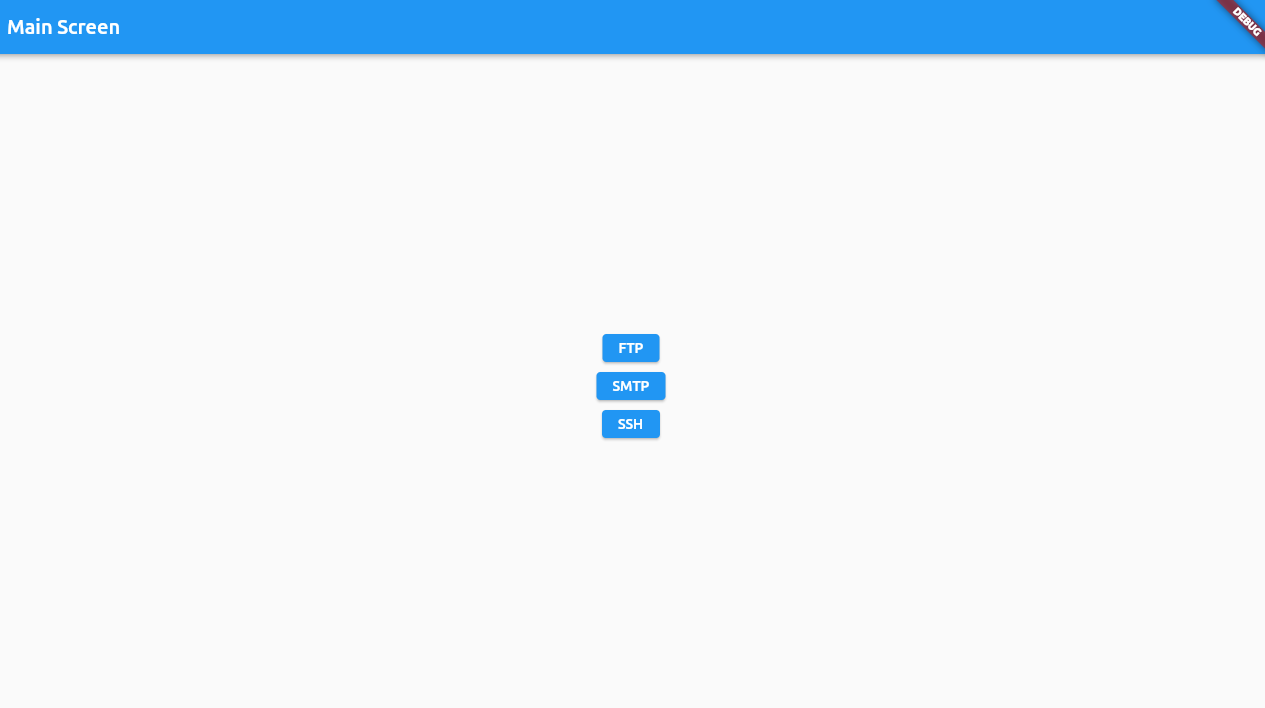
\includegraphics[width=0.8\textwidth]{img1}
\caption{Результаты}
\label{fig:img1}
\end{figure}

\begin{figure}[!htb]
	\centering
	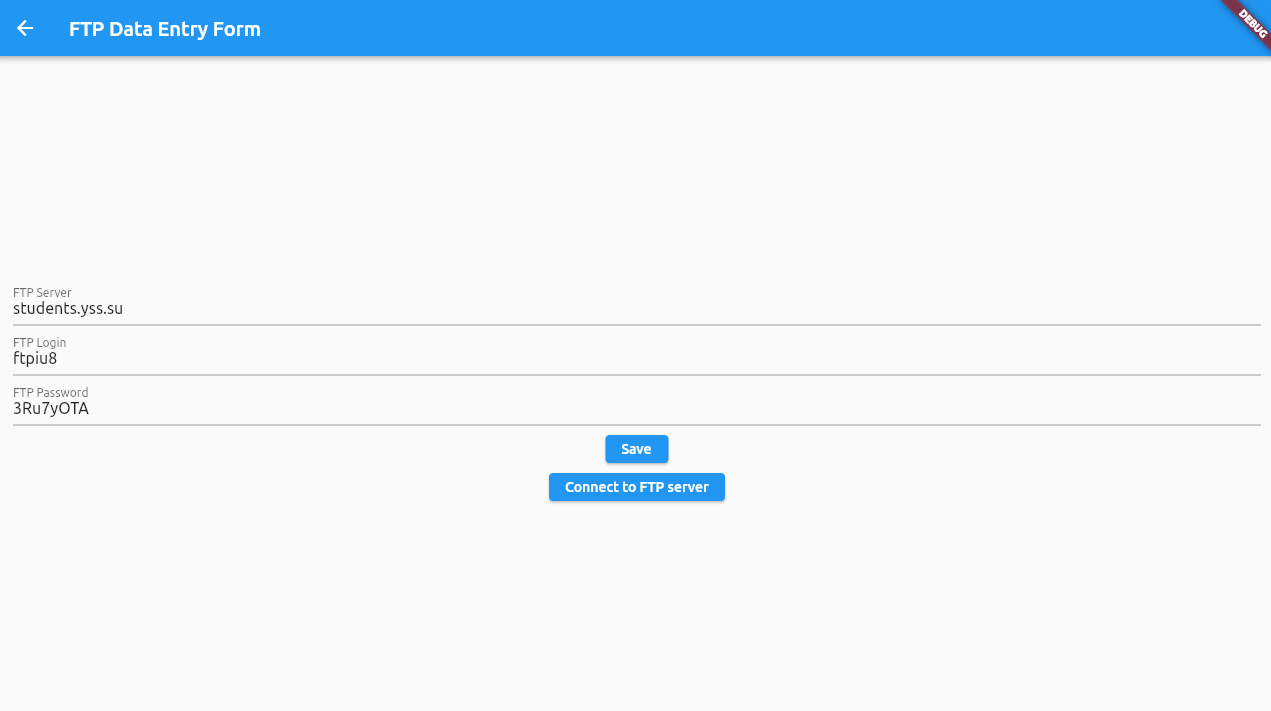
\includegraphics[width=0.8\textwidth]{img2}
\caption{Результаты}
\label{fig:img2}
\end{figure}

\begin{figure}[!htb]
	\centering
	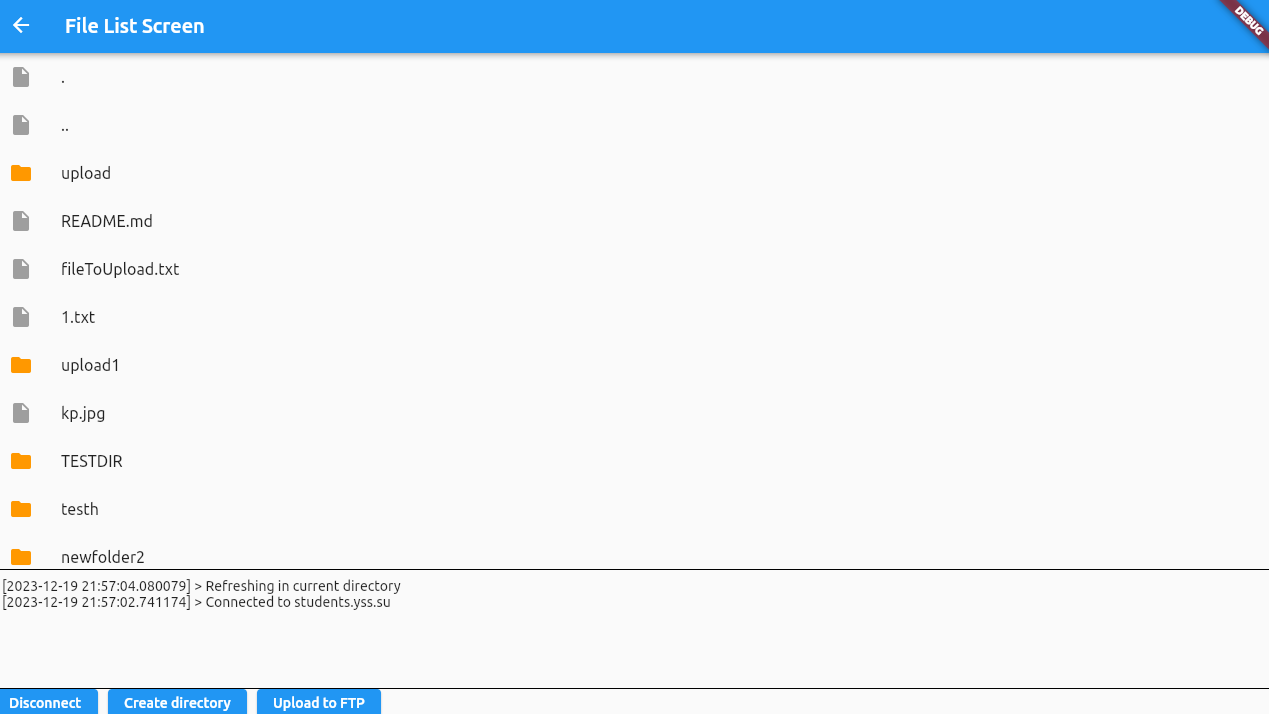
\includegraphics[width=0.8\textwidth]{img3}
\caption{Результаты}
\label{fig:img3}
\end{figure}

\begin{figure}[!htb]
	\centering
	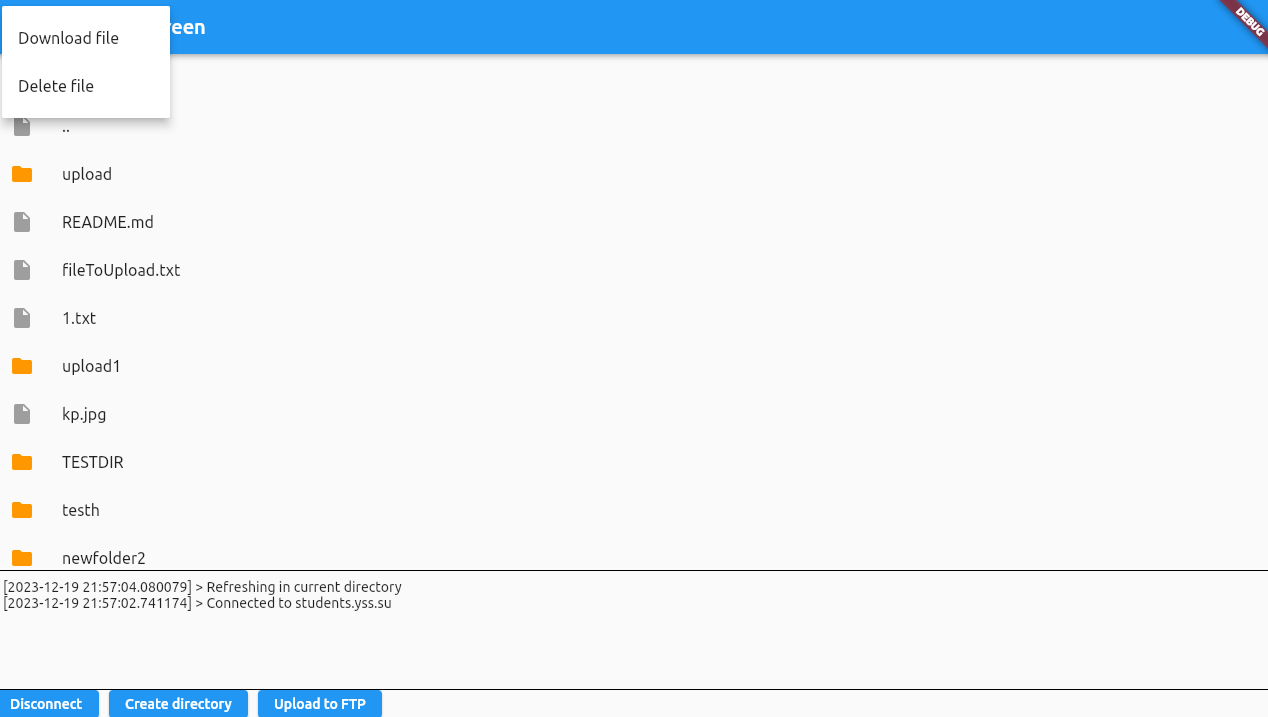
\includegraphics[width=0.8\textwidth]{img4}
\caption{Результаты}
\label{fig:img4}
\end{figure}

\begin{figure}[!htb]
	\centering
	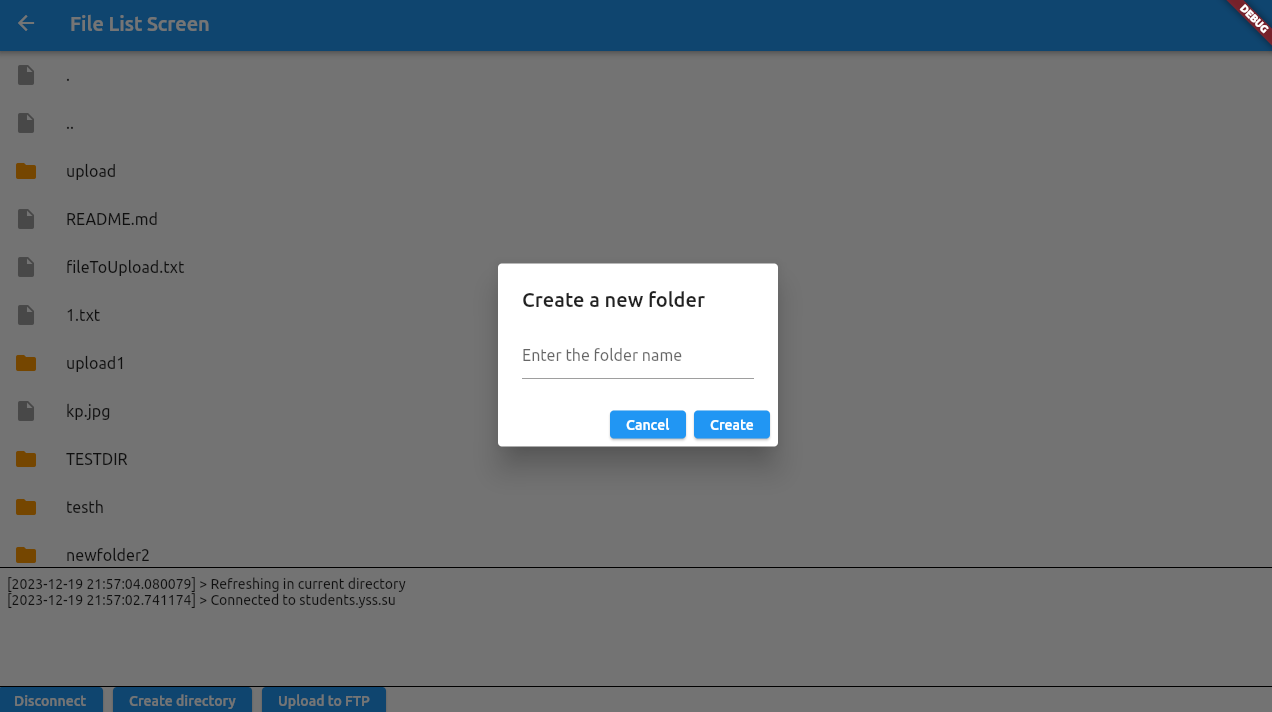
\includegraphics[width=0.8\textwidth]{img5}
\caption{Результаты}
\label{fig:img5}
\end{figure}

\begin{figure}[!htb]
	\centering
	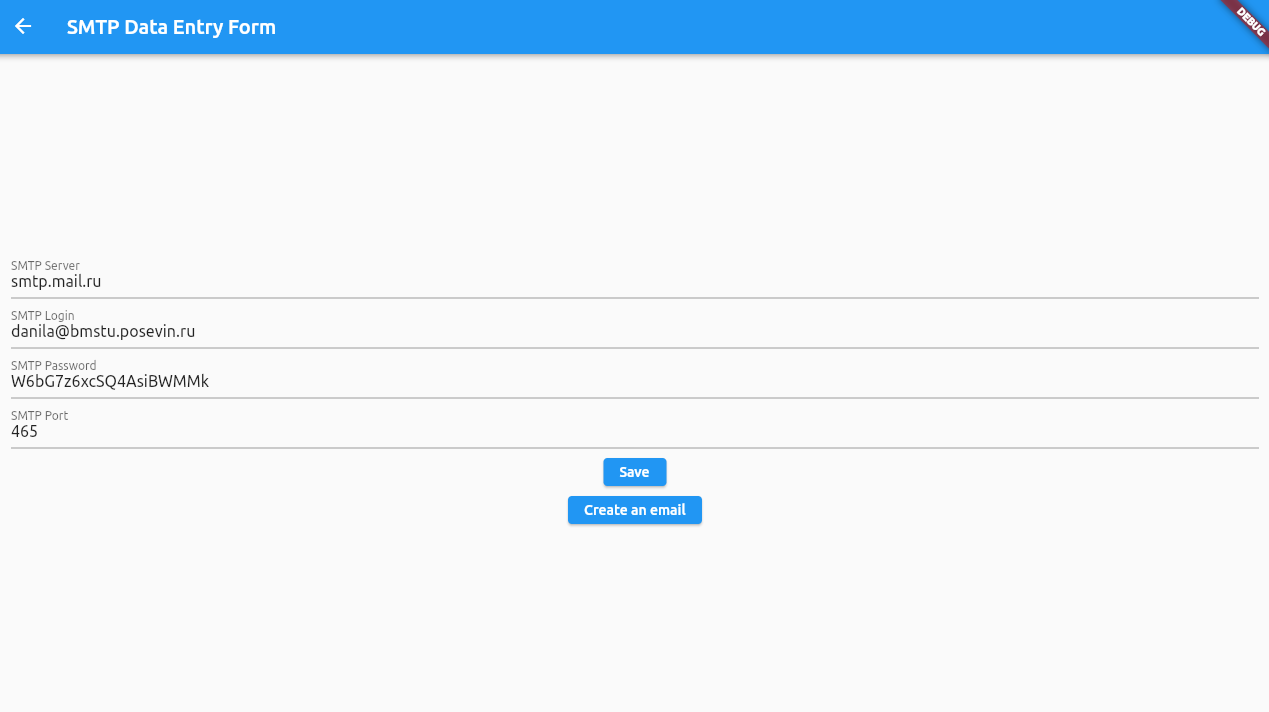
\includegraphics[width=0.8\textwidth]{img6}
\caption{Результаты}
\label{fig:img6}
\end{figure}

\begin{figure}[!htb]
	\centering
	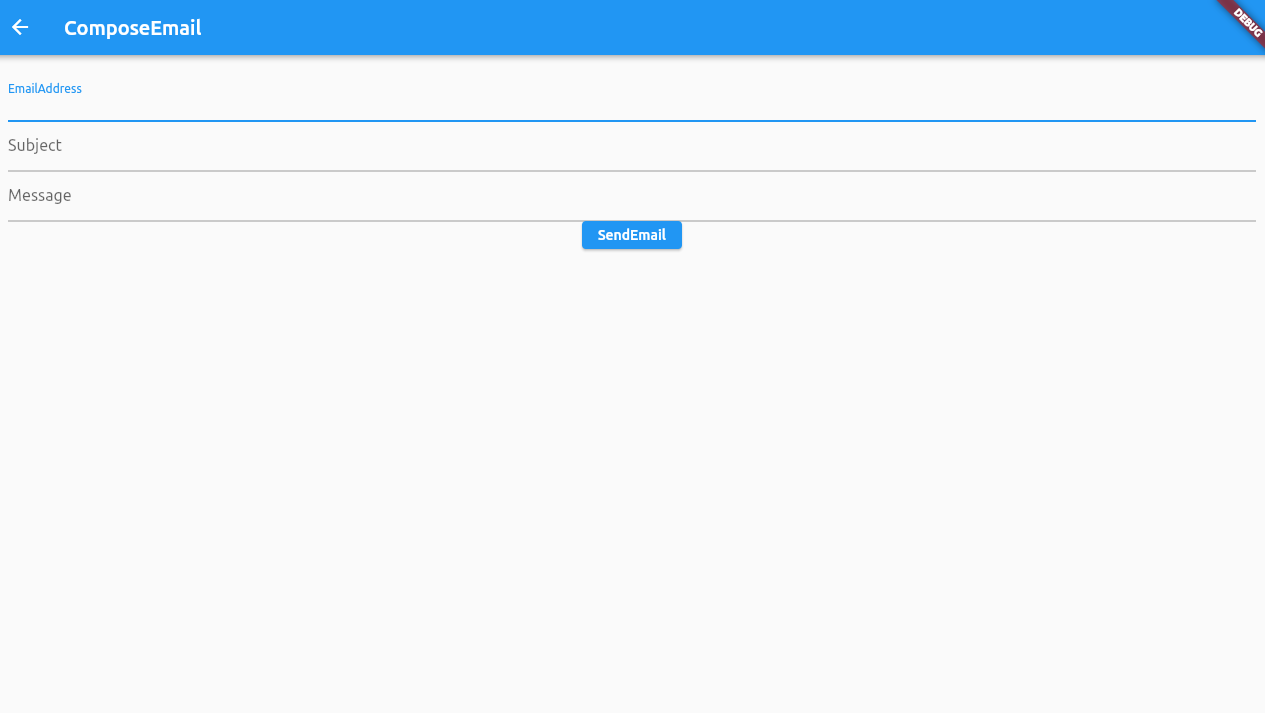
\includegraphics[width=0.8\textwidth]{img7}
\caption{Результаты}
\label{fig:img7}
\end{figure}

\begin{figure}[!htb]
	\centering
	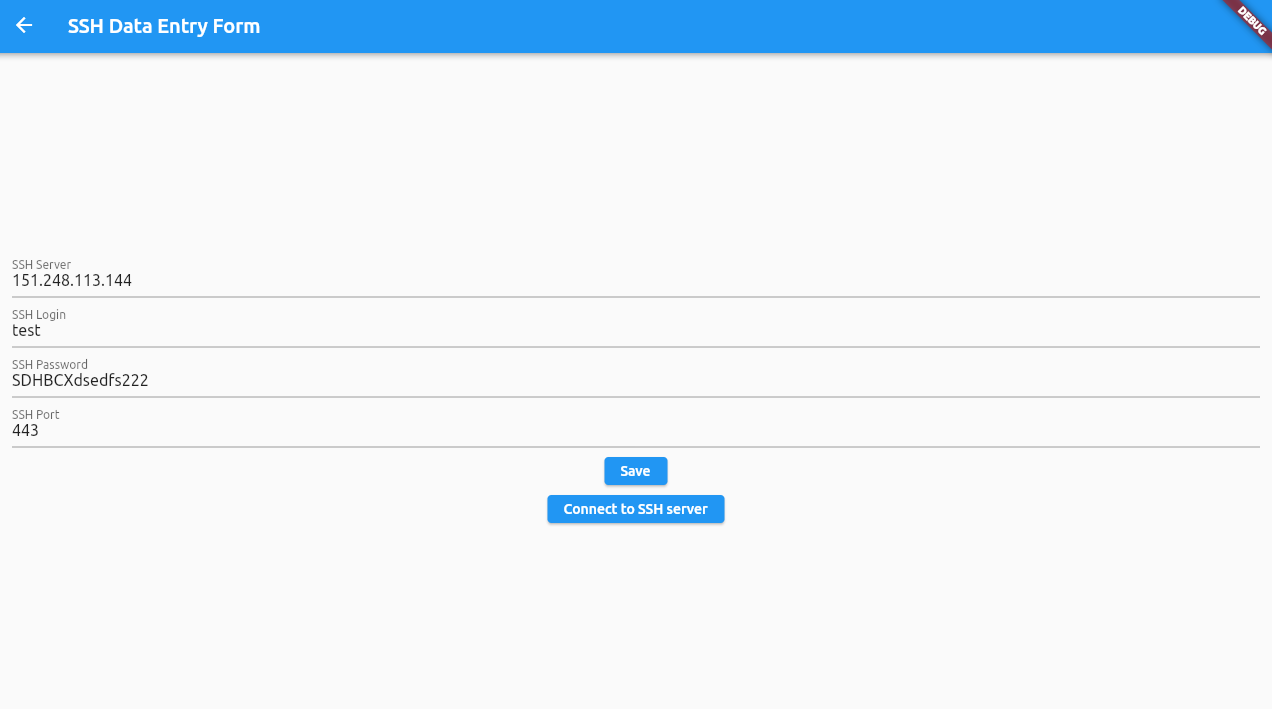
\includegraphics[width=0.8\textwidth]{img8}
\caption{Результаты}
\label{fig:img8}
\end{figure}

\begin{figure}[!htb]
	\centering
	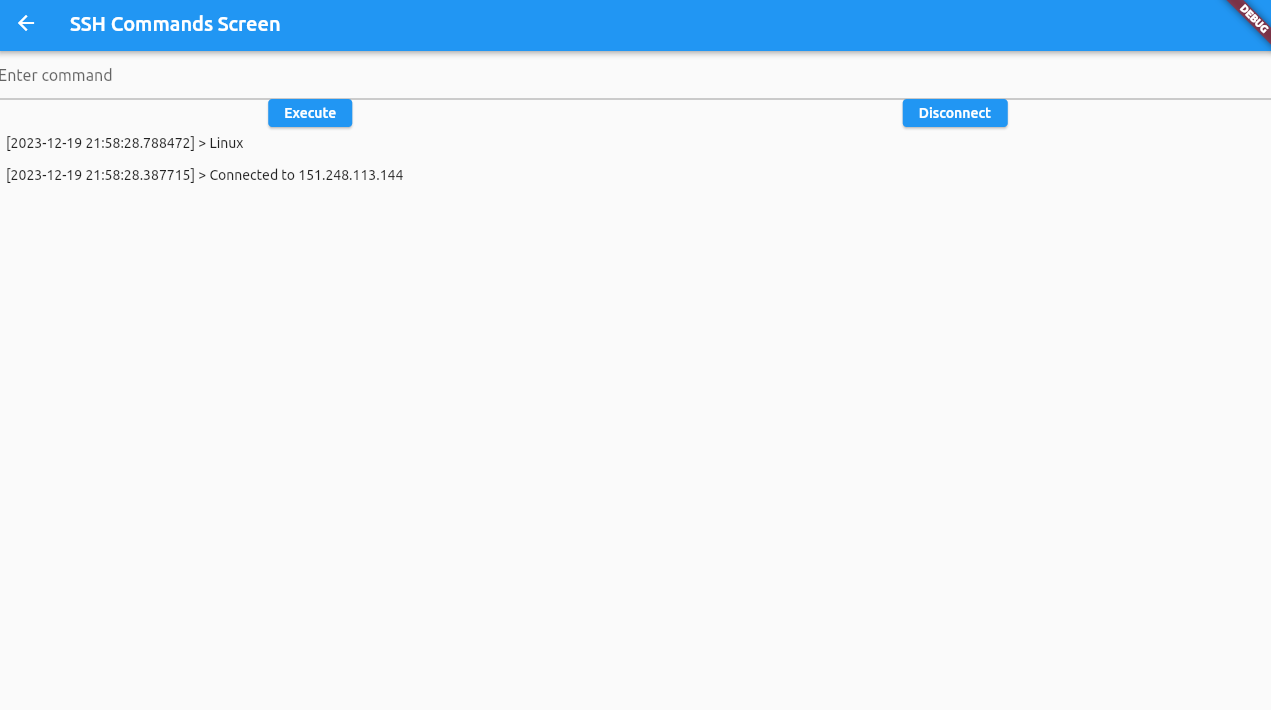
\includegraphics[width=0.8\textwidth]{img9}
\caption{Результаты}
\label{fig:img9}
\end{figure}

\begin{figure}[!htb]
	\centering
	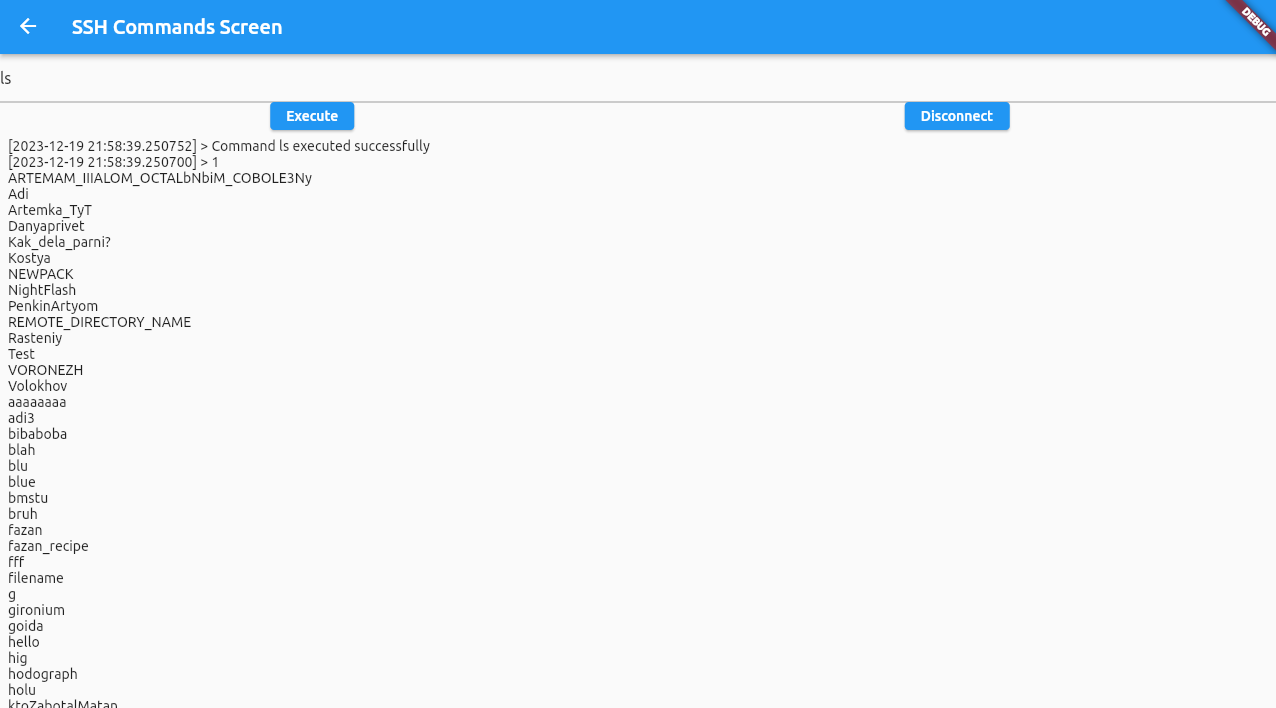
\includegraphics[width=0.8\textwidth]{img10}
\caption{Результаты}
\label{fig:img10}
\end{figure}

\section{Выводы}\label{Sect::conclusion}

В результате выполнения лабораторной работы было реализовано мобильное приложение выполняющее функцию FTP-клиента,  SSH-клиента и SMTP-клиента.

\end{document}